%!TEX TS-program = xelatex
%!TEX encoding = UTF-8 Unicode

\documentclass[12pt]{article}
\usepackage{geometry}                % See geometry.pdf to learn the layout options. There are lots.
\geometry{a4paper,top=2cm}
\usepackage[parfill]{parskip}    % Activate to begin paragraphs with an empty line rather than an indent
\usepackage{graphicx}
\usepackage{amsmath}
\usepackage{amssymb}
\usepackage{mathtools}
\usepackage{physics}
\newcommand{\be}{\begin{equation}}
\newcommand{\ee}{\end{equation}}
\usepackage[thicklines]{cancel}
\usepackage[colorlinks=true,citecolor=blue,linkcolor=blue,urlcolor=blue]{hyperref}
\usepackage{booktabs}
\usepackage{csquotes}
\usepackage{qcircuit}
\usepackage{circledsteps}
\usepackage{nicefrac}
\usepackage{fontspec,xltxtra,xunicode}
\usepackage{xcolor}
\usepackage{simplewick}
\defaultfontfeatures{Mapping=tex-text}

\newcommand{\polv}{\ensuremath{\updownarrow}}
\newcommand{\polh}{\ensuremath{\leftrightarrow}}
\newcommand{\poldr}{\rotatebox[origin=c]{45}{\ensuremath{\leftrightarrow}}}
\newcommand{\poldl}{\rotatebox[origin=c]{-45}{\ensuremath{\leftrightarrow}}}
\newcommand{\bigzero}{\mbox{\normalfont\Large\bfseries 0}}
\newcommand{\vecrp}{\ensuremath{\vec{r}^{\,\prime}}}
\newcommand{\vecnr}{\ensuremath{\vec{\nabla}_{\!r}}}

\title{Advanced Quantum Mechanics\\Class 03}
%\author{The Author}
\date{March 23, 2023}                                           % Activate to display a given date or no date

\begin{document}
\maketitle

\setcounter{section}{1}
\setcounter{subsection}{7}
\setcounter{equation}{54}

%%% 1 OK

\subsection{Temporal Heisenberg inequalities}

Evolution equation for the expectation value
\be
\langle\hat{A}(t)\rangle=\langle\varphi(t) | \hat{A} | \varphi(t)\rangle
\ee
where $\hat{A}$ represents a physics property $\mathcal{A}$
assumed to be independent of time.
\[
\begin{aligned} \frac{d}{d t}\langle\varphi(t)|\hat{A}| \varphi(t)\rangle 
&=\langle d \varphi / d t|\hat{A}| \varphi\rangle+\langle\varphi|\hat{A}| d \varphi / d t\rangle \\ &=\left\langle\frac{1}{i \hbar} \hat{H} \varphi|\hat{A}| \varphi\right\rangle+\left\langle\varphi|\hat{A}| \frac{1}{i \hbar} \hat{H} \varphi\right\rangle \\ 
&=\frac{1}{i \hbar}\langle\varphi(t)|
\underbrace{(\hat{A}\hat{H}-\hat{H}\hat{A})}%
_{[\hat{A},\hat{H}]}
|\varphi(t)\rangle
\end{aligned}
\]
and therefore
\be
\begin{aligned} 
\frac{d}{d t}\langle\hat{A}\rangle_{\varphi}(t) &=\frac{1}{i \hbar}\langle\varphi(t)|[\hat{A}, \hat{H}]| \varphi(t)\rangle \\ &=\frac{1}{i \hbar}\langle[A, \hat{H}]\rangle_{\varphi} 
\end{aligned}
\ee
and here we use the Heisenberg inequality with $\hat{B} \to \hat{H}$
%%% 2 OK
\[
\left(\Delta_{\varphi} \hat{H}\right)\left(\Delta_{\varphi} \hat{A}\right) \geqslant 
\frac{1}{2}|-i
\underbrace{\langle[\hat{A}, \hat{H}]\rangle_{\varphi}}%
_{i \hbar \frac{d}{d t}\langle\hat{A}\rangle_{\varphi}(t)}
|
\]
and finally
\be
\boxed{
\left(\Delta_{\varphi} \hat{H}\right)\left(\Delta_{\varphi} \hat{A}\right) \geqslant \frac{\hbar}{2}\left|\frac{d}{d t}\langle\hat{A}\rangle_{\varphi}(t)\right|
\label{eq:g57}
}
\ee

Notice that
\be
\frac{1}{(\Delta_{\varphi} A)}\left|\frac{d}{d t}\langle\hat{A}\rangle_{\varphi}(t)\right| 
\equiv 
\frac{1}{\tau_\varphi(A)}
\ee
has dimension of inverse of time.
We can call $\tau_\varphi(A)$ a characteristic time for the
expectation value of $\hat{A}$ to change 
by $\Delta_{\varphi} A$.
So we go back to Eq.~\eqref{eq:g57} and write
\be
\boxed{
\left(\Delta_{\varphi} \hat{H}\right) \tau_{\varphi}(\hat{A}) \geq \hbar / 2
}
\ee
Often written as 
\be
\Delta E \Delta t \geq \hbar / 2
\ee
where
$\Delta E$ is the spread of energy, and 
$\Delta t$ is the characteristic evolution time.

\emph{Important:} status of $\left(\Delta_{\varphi} \hat{A}\right)\left(\Delta_{\varphi} \hat{B}\right) \geqslant 1/2 |\langle\hat{C}\rangle_{\varphi}|$
is different from this equation. There is no
%%% 3 OK
$\hat{T}$ operator for time such that
$[\hat{T},\hat{H}] = i\hbar$.

In $\Delta E \Delta t \geq \hbar / 2$: $\Delta E \neq 0$ means that the energy
\emph{cannot} be fixed exactly. When fixed,
then $\Delta t \to \infty$, ``takes infinite time
to evolve''. This points to a stationary state (atom or
nucleus in ground state, elementary particle, \ldots)
\emph{But}, an atom or a nucleus when raised
to an excited state \emph{is not} in a stationary
state because the electrons, nucleons
interact with an e.m. field.
So the atom, or nucleus, emits a \emph{photon}
after some time interval $\Delta t$:
\be
\genfrac{}{}{0pt}{0}{\text{lifetime of the}}{\text{excited state}} \to \Delta t \equiv \tau
\ee
The energy of the final \emph{photon} has
a spread of energy $\Delta E$:
\be
\genfrac{}{}{0pt}{0}{\text{width of the}}{\text{excited state}} \to \Delta E \equiv \hbar \Gamma
\ee

%%% 4 OK

The decay law of the excited state is approximately
exponential: the \emph{survival probability} $p(t)$
of the excited state is
\be
p(t)=e^{-t / \tau}
\ee
\emph{Exercise 4.4.5:} $\Delta E$ and $\tau$ related by Fourier
transform and $\tau\Delta E \sim \hbar$ leads to
\be
\tau \Gamma \simeq 1
\ee
$\Delta E$ \emph{is not} the same as the dispersion of $\hat{H}$
in an excited state ($\equiv \varphi^*$), $\Delta_{\varphi^*} \hat{H}$.
For the exponential law (\emph{exercise 4.5})
\be
\Delta_{\varphi^*} \hat{H} \gg \Delta E=\hbar \Gamma
\ee

\emph{An application of} $\Delta E \Delta t \geqslant \hbar / 2$: 

\begin{center}
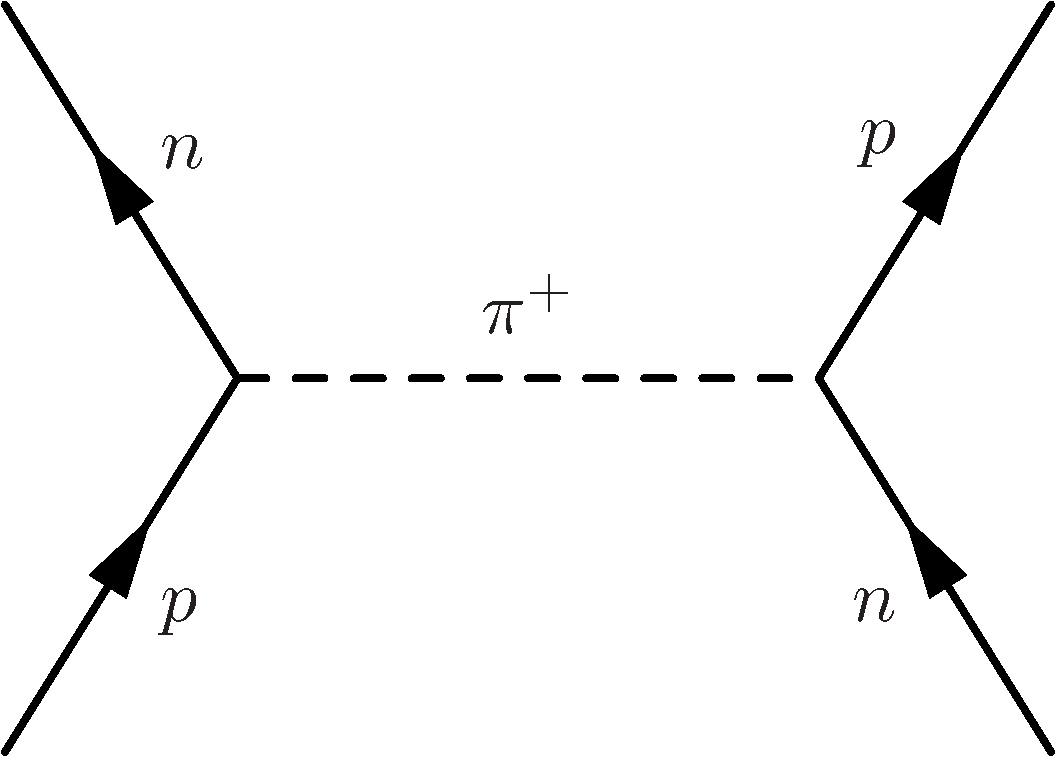
\includegraphics[height=8em]{Figures/np-piplus-pn.pdf}\quad\quad%
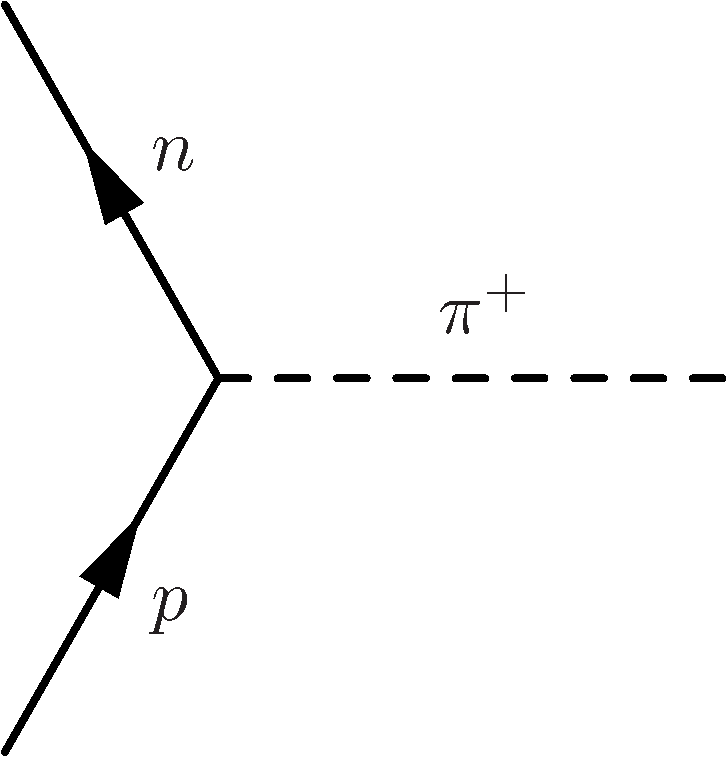
\includegraphics[height=8em]{Figures/np-piplus.pdf}
\end{center}

The process in the right
does not conserve 
simultaneously
energy and
momentum
-- cannot happen
in free space.

But the $\pi^+$ can propagate for a short time $\Delta t$
if its energy fluctuates by an amount
\be
\Delta E \simeq \frac{\hbar}{\Delta t}
\ee
%%% 5 OK
and after that is absorbed by the neutron.
This fluctuation is of the order of the mass
of the $\pi^+$: $\Delta E \sim m_{\pi^+}+c^{2}$.
How far has it travelled during this time?
We can calculate the maximum distance:
\be
r \sim \Delta t c \sim \frac{\hbar c}{\Delta E} \simeq \frac{\hbar c}{m_{\pi} c^{2}} \simeq \frac{200\, \text{MeV}\,\text{fm}}{140\,\text{MeV}} \sim 1.5\,\text{fm}
\ee
and $r$ can be identified with the range of the nuclear force.
Yukawa (1935) knew $r$ $\to$ predicted $m_\pi \simeq 200\,\text{MeV}$.


\subsection{Schrödinger and Heisenberg pictures}

So far, dynamics was supposed to be
carried by the state vectors $\ket{\varphi(t)}$.
This is the Schrödinger picture.

At the end of the day, contact with experiment
is made through scalar products and
matrix elements
\[
\langle\varphi|\hat{A}| \psi\rangle(t)
\]
where the $t$ dependance can be 
in $\ket{\varphi}$ or $\ket{\psi}$
or in $\hat{A}$.

%%% 6 OK

Simplify the discussion, consider $\hat{H}$ and $\hat{A}$
both independent of time:
\[
\begin{aligned}
\langle A\rangle_{\varphi}(t) 
&=\langle\varphi(t)|\hat{A}| \varphi(t)\rangle \\ 
&=\langle\varphi(t_{0})
|
\underbrace{
e^{i  / \hbar\left(t-t_{0}\right) \hat{H}} 
\hat{A} 
e^{-i / \hbar\left(t-t_{0}\right) \hat{H}}
}%
_{\hat{A}_H(t)}
| 
\varphi(t_{0})\rangle
\end{aligned}
\]
where we define $\hat{A}_H(t)$, the operator $\hat{A}$ in the Heisenberg picture as:
\be
\begin{aligned} 
\hat{A}_{H}(t) &=e^{i / \hbar\left(t-t_{0}\right) \hat{H}} \hat{A} e^{-i / \hbar\left(t-t_{0}\right) \hat{H}} \\ 
&=\hat{U}^{\dagger}\left(t, t_{0}\right) \hat{A} \, \hat{U}\left(t, t_{0}\right)
\end{aligned}
\ee
and hence the time-dependent expected value is
\be
\langle A\rangle_{\varphi}(t)=\left\langle\varphi\left(t_{0}\right)\left|\hat{A}_{H}(t)\right| \varphi\left(t_{0}\right)\right\rangle
\ee

\emph{Exercise 4.4.7:} Suppose $\hat{A} = \hat{A}(t)$, $\hat{H} = \hat{H}(t)$.
Show that
\be
\hat{A}_{H}(t)=\hat{U}^{-1}\left(t, t_{0}\right) \hat{A}(t) \hat{U}\left(t, t_{0}\right)
\label{eq:g70}
\ee
satisfies the Heisenberg equation of motion:
\be
i \hbar \frac{d}{d t} \hat{A}_{H}(t)=\left[\hat{A}_{H}(t), \hat{H}_{H}(t)\right]+i \hbar\left(\frac{\partial A(t)}{\partial t}\right)_{H}
\ee
where $\hat{H}_{H}(t)$ and $\left(\frac{\partial A(t)}{\partial t}\right)_{H}$ are obtained 
from $\hat{H}(t)$ and $\left(\frac{\partial A(t)}{\partial t}\right)$ by the transformation
law in Eq.~\eqref{eq:g70}.

%%% 7 OK

\subsection{Approximations and modelling} 

The general principles that define the universal
framework of quantum physics
are not enough to tackle
a physical system, one needs to
specify a space of states and a
Hamiltonian: they depend on the
degree of precision we aim at
$\to$ simplifications, approximations (\emph{model}).
NOT to be confused with the general principles.

\emph{Examples:}
 
\begin{enumerate}
\item spin-1/2 decoupled from its spatial
degrees of freedom $\to$ 2-dim. space.
\item two level atom: when interested in
the interaction between an atom and
an e.m. field of frequency $\omega$ (laser)
$\to$ if spacing of two energy levels 
$E_2-E_1 \simeq \hbar \omega$, one can limit
discussion to the levels $E_1$ and $E_2$,
again a 2-dim. space.
Notice that this is an excellent approximation 
for the laser-atom interaction
\end{enumerate}

%%% 8 OK

It is not always so easy, we will see more in \emph{Chapter 9}.

Spatial degrees of freedom can be dealt with
use of the \emph{correspondence principle:}
classical variables $\mathbf{r} = (x,y,z)$, $\mathbf{p} = (p_x,p_y,p_z)$.
We promote the variables to operators:
$\mathbf{r} \to \hat{\mathbf{r}}$,
$\mathbf{p} \to \hat{\mathbf{p}}$,
and impose the commutation relations:
\be
[x_i,p_j] = i\hbar \delta_{ij}I,\quad i=x,y,z
\ee
Take trace on both sides of this equation
\[
\operatorname{Tr}\left[x_{i}, p_{j}\right]=0,\quad \operatorname{Tr} \delta_{i j} I \neq 0
\]
for a finite-dimensional space.
Need to consider infinite dimension Hilbert space.

Once this is recognised: classical $\to$ quantum
\be
E \rightarrow \hat{H},\quad \mathbf{r} \rightarrow \hat{\mathbf{r}},\quad \mathbf{p} \rightarrow \hat{\mathbf{p}}
\ee
\be
E=\frac{\mathbf{p}^{2}}{2 m}+V\left(\mathbf{r}\right) 
\rightarrow 
\hat{H}=\frac{\hat{\mathbf{p}}^{2}}{2 m}+V\left(\hat{\mathbf{r}}^{2}\right)
\label{eq:g74}
\ee
and it is a very good approach to the hydrogen atom
if using Coulomb potential
for $V(\mathbf{r})$.
If the proton is infinitely heavy $\to$ $m$ in Eq.~\eqref{eq:g74} is $m_e$.
If the proton has finite mass $\to$
\be
m = \frac{m_{p} m_{e}}{m_{p}+m_{e}}=\mu
\ee 

%%% 9 OK

Relativistic effects $\to$ complications
\begin{itemize}
\item Dirac equation, 1\textsuperscript{st} step: 
relativistic correction to the kinetic energy,
spin-orbit coupling (with Thomas precession, frame shift from nucleus frame to electron frame),
Darwin term.
\item QFT, effects like Lamb shift and anomalous magnetic dipole moment.
In particular, this leads to QED: no position operator.
\end{itemize}
But QED is also an approximation!

\begin{center}
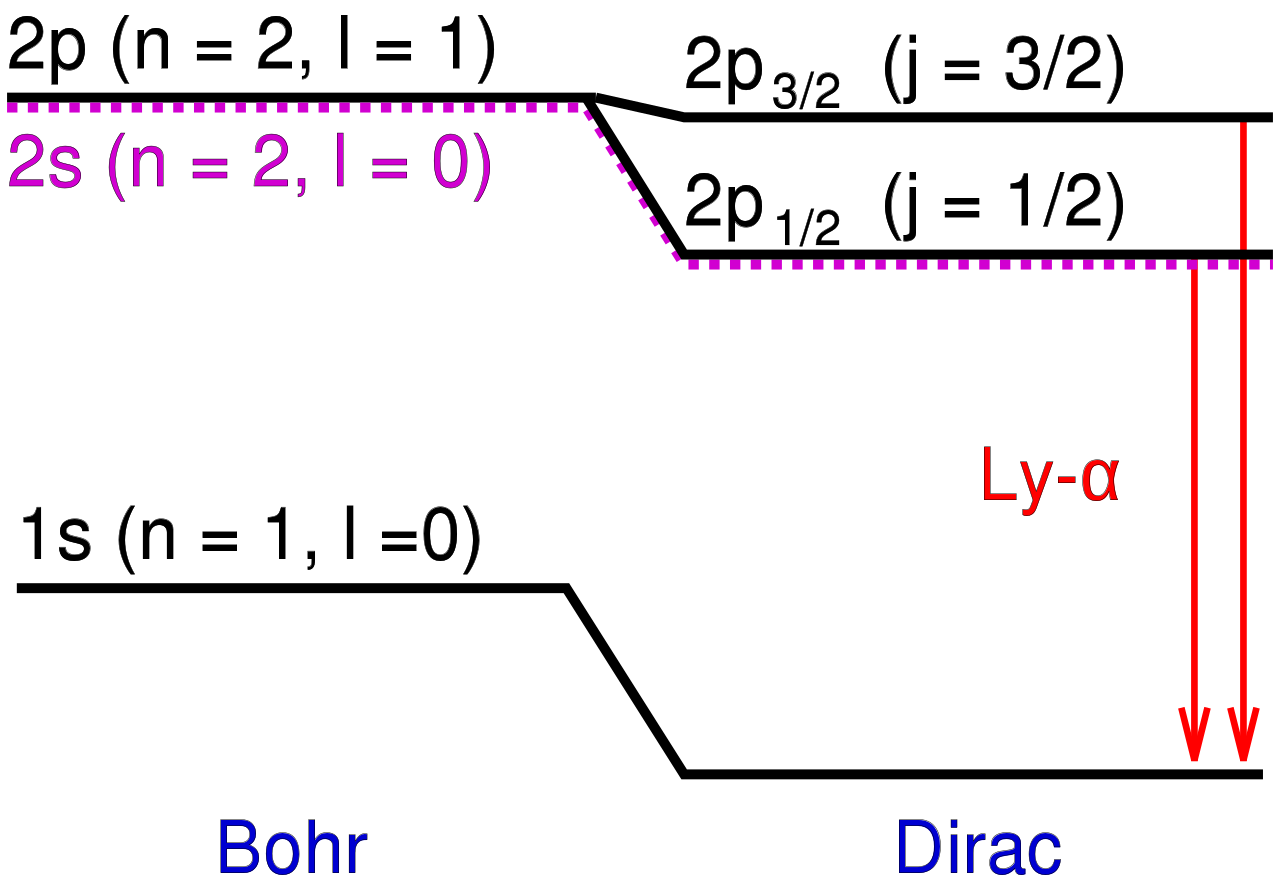
\includegraphics[width=0.5\textwidth]{Figures/1280px-Hydrogen-fine-structure2.png}
\\Bohr model, Dirac corrections. The Lamb shift is the difference between the 
$2s_{1/2}$ (dotted purple)
and
$2p_{1/2}$ (solid black) in the right.
\end{center}

\emph{Bottom line:} quantising a classical theory
using the correspondence principle has
only heuristic value (Isham $\to$ see ref. in Le Bellac 
or \href{https://isbnsearch.org/isbn/9781860940019}{click here}).
In the end, the approximations based 
on this principle or other heuristic
approach must be validated by confronting
with experimental results.

$\mathcal{A}$ physical property, $\hat{A}$ operator representing
this in $H$: from here on, \emph{abandon} the
differentiation, unless explicitly stated.
\emph{BUT:} property and operator by capital 
letters $\hat{H}$, $\hat{\mathbf{R}}$, $\hat{\mathbf{P}}$ with a hat.
Eigenvalues $\hat{H} \to E$, $\hat{\mathbf{R}} \to \mathbf{r}$, $\hat{\mathbf{P}} \to \mathbf{p}$.


































\end{document}  